\chapter{Literature Review}
\section{Ch2\_Sec1}
\lipsum[1]

In Figure~\ref{fig:eirf}, feature f1 is a relevant because it is able to identify natural groups of the data in Figure~\ref{fig:eirf}a. Feature f2 in Figure~\ref{fig:eirf}b, is an irrelevant feature because it is not able to identify natural groups of the data. Figure~\ref{fig:eirf}c shows the impact of irrelevant / noisy feature on the learning algorithm (Clustering algorithm). In the presence of irrelevant features, the similarity between objects represented by the feature space may not truly reflect the memberships of data objects to classes.

\begin{center}
\begin{figure}
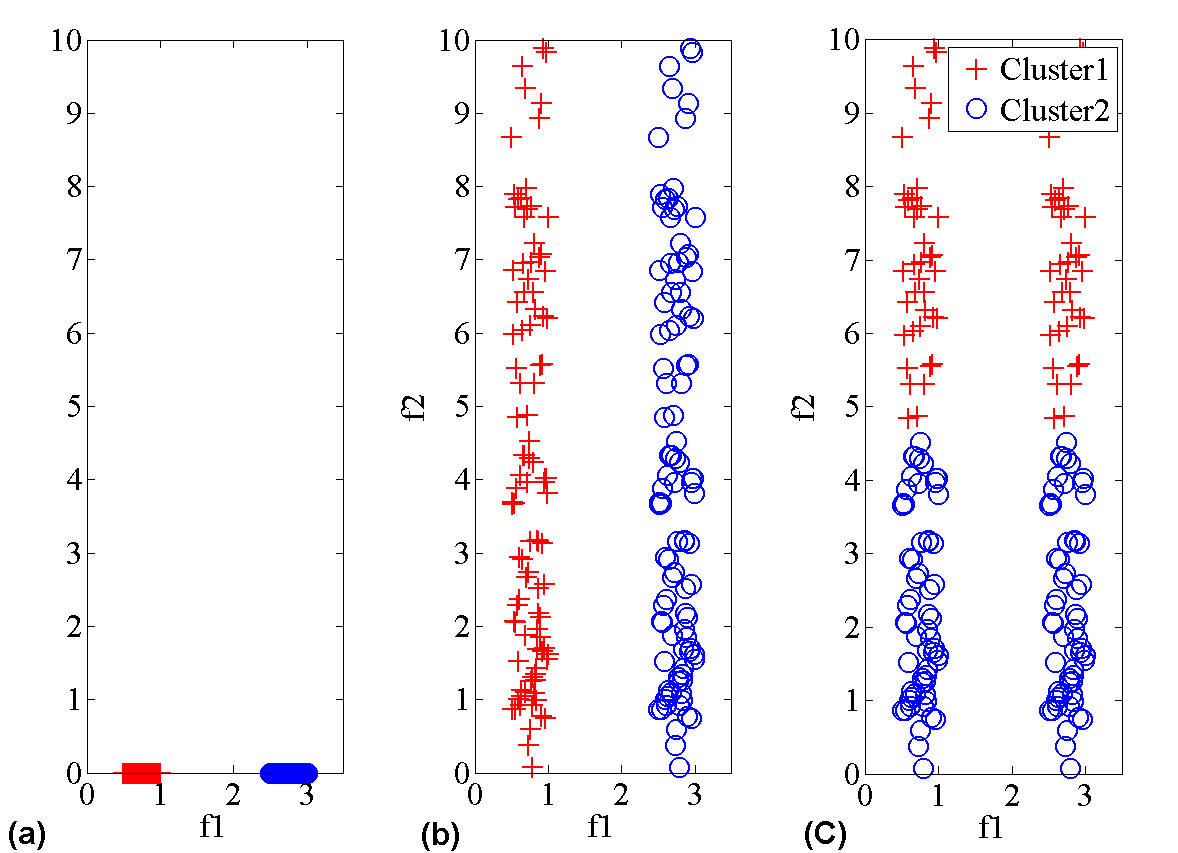
\includegraphics[scale=0.5]{images/irrelavent.png}
\caption{Impact of irrelevant feature on Clustering quality}
\label{fig:eirf}
\end{figure}
\end{center}



The equation of a circle is shown in Eq.~(\ref{eq:cir}).

\begin{equation}
x^2+y^2=1 
\label{eq:cir}
\end{equation} 
 
The equation of an ellipse is defined in  Eq.~(\ref{eq:ell}).
\begin{equation}
\frac{x^2}{a^2} + \frac{y^2}{b^2} = 1
\label{eq:ell}
\end{equation}

where $a$ is the semi-major axis and $b$ is the semi-minor axis.

\section{Ch2\_Sec2}

A feature in a pair of features is redundant, if they co-occur with each other and are relevant individually, however elimination of one feature in the pair does not deteriorate clustering performance \cite{yu2004}. The distribution of credits across semesters in R20 curriculum for BTech in Information Technology is shown in Table~\ref{Tab:doc}.

\begin{minipage}{\textwidth}
\centering
\captionof{table}{Distribution of credits across semesters}
\begin{tabular}{lcc}
\toprule 
\multirow{2}{*}{Semester}	&	\multicolumn{2}{c}{Credits}\\	
\cmidrule{2-3}
                           & Proposed & APSCHE \\ 
\midrule
I 				& 19.0		& 19.5 \\

II 				& 20.0		& 19.5 \\

III 			& 22.5		& 21.5 \\

IV 				& 20.5		& 21.5 \\

V 				& 22.0		& 21.5 \\

VI 				& 21.5		& 21.5 \\

VII 			& 22.5		& 23.0 \\

VIII 			& 12.0		& 12.0 \\
\midrule
Total			& 160       & 160 \\ 
\bottomrule
\end{tabular}
\label{Tab:doc}
\end{minipage}

\section{Ch2\_Sec3}

After a student has satisfied the requirements prescribed for the completion of the program and is eligible for the award of B. Tech. degree, he/she shall be placed in one of the following four classes as shown in Table~\ref{Tab:cls}.

\begin{minipage}{\textwidth}
\centering
\captionof{table}{Award of class based on obtained CGPA}
\begin{tabular}{ll}
\toprule
\textbf{Class Awarded}	& \textbf{CGPA Secured} \\
\midrule
First Class with Distinction &	≥ 7.5 \\
First Class	& ≥ 6.5 < 7.5 \\
Second Class &	≥ 5.5 < 6.5 \\
Pass Class	& ≥ 4.0 < 5.5 \\
\bottomrule
\end{tabular}
\label{Tab:cls}
\end{minipage}






